\documentclass{beamer}
%Imports and customization
\usepackage{tikz}
\usepackage{graphicx}
\usepackage{tikz-feynman}
\usepackage{ulem}
\usepackage{colortbl}
\graphicspath{ 
    {./images/}
}

\beamertemplatenavigationsymbolsempty
\setbeamertemplate{sidebar right}{}
\setbeamertemplate{footline}{
    \hfill\usebeamertemplate***{navigation symbols}
    \hspace{1cm}\insertframenumber{}/\inserttotalframenumber
}
\setbeamertemplate{caption}{\raggedright\insertcaption\par}
\setbeamersize{text margin left=4mm,text margin right=4mm} 

\setbeamerfont{itemize/enumerate body}{size=\scriptsize}
\setbeamerfont{itemize/enumerate subbody}{size=\scriptsize}
\setbeamerfont{itemize/enumerate subsubbody}{size=\scriptsize}


%Custom Macros
\newcommand{\statwarn}{
    \tiny \color{red} Absolute numbers here mean NOTHING. Plots are based on small (100k events) samples, and are highly biased. All that matters is relative position!
}


% WARNING: When using these commands, the image argument must
% NOT have spaces between itself and the braces
\newcommand{\fullscreenimage}[2]{
    \frame{
        \frametitle{#1} 
        \begin{figure}
        \includegraphics[height=0.9\textheight,width=\textwidth,keepaspectratio]{#2}
        \end{figure}
    }
}


\newcommand{\importpdf}[3]{
    \frame{
        \begin{columns}\column{\dimexpr\paperwidth-10pt}
        \begin{figure}
        \includegraphics[page=#2,height=0.8\textheight,width=\textwidth,keepaspectratio]{#1}
        \end{figure}

        {\tiny #3}
        \end{columns}
    }
}


\newcommand{\displayone}[3]{
    \frame{
        \frametitle{#1} 
        \begin{columns}
            \begin{column}{0.5\textwidth}
                #2
            \end{column}
            \begin{column}{0.5\textwidth}
                \begin{figure}
                    \includegraphics[width=\linewidth,height=\textheight,keepaspectratio]{#3}
                \end{figure}
            \end{column}
        \end{columns}
    }
}

\newcommand{\displayonelarge}[3]{
    \frame{
        \frametitle{#1} 
        \begin{columns}
            \begin{column}{0.3\textwidth}
                #2
            \end{column}
            \begin{column}{0.7\textwidth}
                \begin{figure}
                    \includegraphics[width=\linewidth,height=0.8\textheight,keepaspectratio]{#3}
                \end{figure}
            \end{column}
        \end{columns}
    }
}


\newcommand{\displaytwo}[4]{
    \frame{
        \frametitle{#1} 
        #2
        \begin{columns}
            \begin{column}{0.5\textwidth}
                \begin{figure}
                    \includegraphics[width=\linewidth,height=\textheight,keepaspectratio]{#3}
                \end{figure}
            \end{column}
            \begin{column}{0.5\textwidth}
                \begin{figure}
                    \includegraphics[width=\linewidth,height=\textheight,keepaspectratio]{#4}
                \end{figure}
            \end{column}
        \end{columns}
    }
}

\newcommand{\displaytwocaption}[6]{
    \frame{
        \frametitle{#1} 
        #2
        \begin{columns}
            \begin{column}{0.5\textwidth}
                \begin{figure}
                    \includegraphics[width=\linewidth,height=\textheight,keepaspectratio]{#3}
                    \caption{#4}
                \end{figure}
            \end{column}
            \begin{column}{0.5\textwidth}
                \begin{figure}
                    \includegraphics[width=\linewidth,height=\textheight,keepaspectratio]{#5}
                    \caption{#6}
                \end{figure}
            \end{column}
        \end{columns}
    }
}

\newcommand{\displaytwoVcaption}[6]{
    \frame{
        \begin{columns}
            \begin{column}{0.5\textwidth}
                \frametitle{#1} 
                #2
            \end{column}
            \begin{column}{0.5\textwidth}
                \begin{figure}
                    \includegraphics[width=\linewidth,height=0.3\textheight,keepaspectratio]{#3}
                    \caption{#4}
                \end{figure}

                \begin{figure}
                    \includegraphics[width=\linewidth,height=0.3\textheight,keepaspectratio]{#5}
                    \caption{#6}
                \end{figure}
            \end{column}
        \end{columns}
    }
}


\newcommand{\displaythree}[5]{
    \frame{
        \begin{columns}[T]
            \begin{column}{0.4\textwidth}
                {\usebeamercolor[fg]{title} \insertframetitle{#1} }\\
                \vspace{5mm}
                #2
            \end{column}
            \begin{column}{0.4\textwidth}
                \begin{figure}
                    \includegraphics[width=\linewidth,height=\textheight,keepaspectratio]{#3}
                \end{figure}
            \end{column}
        \end{columns}
        \begin{columns}[T]
            \begin{column}{0.4\textwidth}
                \begin{figure}
                    \includegraphics[width=\linewidth,height=\textheight,keepaspectratio]{#4}
                \end{figure}
            \end{column}
            \begin{column}{0.4\textwidth}
                \begin{figure}
                    \includegraphics[width=\linewidth,height=\textheight,keepaspectratio]{#5}
                \end{figure}
            \end{column}
        \end{columns}
    }
}


\newcommand{\displayfour}[5]{
    \frame{
        \frametitle{#1} 
        \begin{columns}[T]
            \begin{column}{0.4\textwidth}
                \begin{figure}
                    \includegraphics[width=\linewidth,height=\textheight,keepaspectratio]{#2}
                \end{figure}
            \end{column}
            \begin{column}{0.4\textwidth}
                \begin{figure}
                    \includegraphics[width=\linewidth,height=\textheight,keepaspectratio]{#3}
                \end{figure}
            \end{column}
        \end{columns}
        \begin{columns}[T]
            \begin{column}{0.4\textwidth}
                \begin{figure}
                    \includegraphics[width=\linewidth,height=\textheight,keepaspectratio]{#4}
                \end{figure}
            \end{column}
            \begin{column}{0.4\textwidth}
                \begin{figure}
                    \includegraphics[width=\linewidth,height=\textheight,keepaspectratio]{#5}
                \end{figure}
            \end{column}
        \end{columns}
    }
}


\newcommand{\pstrike}[2]{
    \only<-\the\numexpr#1-1>{#2}
    \only<#1->{\sout{#2}}
}


\newcommand{\announcesection}[1]{
    \section{#1}
    \frame{
        \begin{center}
            {\huge #1} 
        \end{center}
    }
}

\newcommand{\kvv}{\kappa_{2V}}
\newcommand{\kl}{\kappa_{\lambda}}
\newcommand{\kv}{\kappa_{V}}

\newcommand{\fkvv}[1]{\kappa_{2V,#1}}
\newcommand{\fkl} [1]{\kappa_{\lambda,#1}}
\newcommand{\fkv} [1]{\kappa_{V,#1}}

\newcommand{\importpdfwpages}[3]{
    \foreach \pageN in {#2,...,#3}{
        \importpdf{#1}{\pageN}{}
    }
}

\newcommand{\hyper}[2]{{\color{blue}\href{#1}{#2}}}



%Begin Presentation
\begin{document}
    \title{ Status Report: Online Monitoring and Di-Higgs Analysis }
    \author{Chris Milke}
    \date{18 May, 2020}

    \frame{\titlepage}
    \frame{\frametitle{Overview} \tableofcontents}

    \section{Online Monitoring Migration}
\fullscreenimage{B-Jet Trigger Online Monitoring: I Have a TestBed Account!}{testbed}

    % reiterate basic background and goal
    % show cutflow chart (VBF=1 vs ggF) and explain what's happening. point out where I care
    % note the huge number of ggF events getting through. My goal is to reduce this
    % Show the varied c2v value chart, if only because I made it. Through the kinematics in backup
    % Roc curve time! Use mjj distro and cumalitive distro to explain how I made roc curves
    % Now show the unweighted roc curves to show the different performances
    % Show my BDT
    % Now dissapoint everyone with the weighted version... hey steve, how do I weight stuff in SKlearn BDTs?
    \section{ Di-Higgs Analysis }
\fullscreenimage{VBF Di-Higgs Analysis}{vbf-hh_diagrams}
\frame{
    \frametitle{ VBF $\rightarrow$ HH $\rightarrow$ \fourB }

    \begin{columns}
        \begin{column}{0.5\textwidth}
            { \small
                Goal is to put a better limit on the $C_{2V}$ coupling constant.
            }

            \begin{figure}
                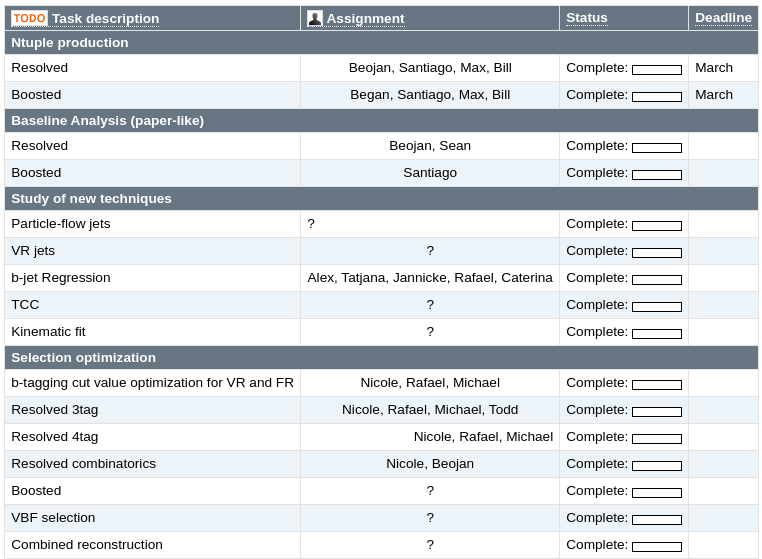
\includegraphics[width=\linewidth,height=\textheight,keepaspectratio]
                {dihiggs_task_list}
            \end{figure}
        \end{column}
        \begin{column}{0.5\textwidth}
            \resizebox{0.50\textheight}{!}{
                \resizebox{.8\textwidth}{!}{
\begin{tikzpicture} \begin{feynman}
    \vertex (c2v) {???};
    \vertex [above right=of c2v] (h1) {$h_1$};
    \vertex [below right=of c2v] (h2) {$h_2$};
    \vertex [above left=of c2v] (vb1);
    \vertex [below left=of c2v] (vb2);
    \vertex [left=of vb1] (q1) {$q_1$};
    \vertex [left=of vb2] (q2) {$q_2$};
    \vertex [above right=of h1] (b1) {$b$};
    \vertex [below right=of h2] (bbar2) {$\bar b$};
    \vertex [below=of b1] (bbar1) {$\bar b$};
    \vertex [above=of bbar2] (b2) {$b$};

    \vertex [above=of b1] (q3) {$q_3$};
    \vertex [below=of bbar2] (q4) {$q_4$};

    \diagram* {
        (q1) -- (vb1) -- (q3),
        (q2) -- (vb2) -- (q4), 
        (vb1) -- [boson] (c2v) -- [boson] (vb2),
        (h1) -- [scalar] (c2v) -- [scalar] (h2),
        (b1) -- (h1) -- (bbar1),
        (b2) -- (h2) -- (bbar2),
    };
\end{feynman} \end{tikzpicture}
}

            }
        \end{column}
    \end{columns}
}

\section{Analysis Baseline Status}

\displayonelarge{VBF Selection Process Overview}{
    Ultimate goal is reducing the ratio of ggF events to VBF events. Focus so far has been in the ``VBF dEta'' and ``VBF mjj'' selection steps.
}{cutflows/general}

\displayonelarge{Current VBF/ggF Separation Performance}{
    Current VBF/ggF separation is achieved using a BDT with inputs:

    \vspace{10mm}

    \begin{itemize} {
        {\tiny \item \mjj of leading \mjj jet pair }
        {\tiny \item \dEta of leading \mjj jet pair }
        {\tiny \item First 7 Fox-Wolfram moments of all non-b-tagged jets}
    } \end{itemize}
}{rocs/current_roc}


\fullscreenimage{ROC Curves!}{roc_explanation}
\fullscreenimage{Comparing Selection Performance}{roc_explanation}
\fullscreenimage{Current Selection Method Performance}{rocs/rocs_initial}

\displayonelarge{Baseline BDT}{
    As a baseline, train BDT with same inputs as current algorithm. It should perform at least as well.
}{rocs/rocs_bdt1}

\fullscreenimage{Adding Fox-Wolfram Moments to BDT}{fwMoment_ordering}
\displayfour{Fox-Wolfram Distributions}
{fw_moments/fox-wolfram_1}
{fw_moments/fox-wolfram_2}
{fw_moments/fox-wolfram_3}
{fw_moments/fox-wolfram_4}


\displaytwo{BDT with Fox-Wolfram Moments}{
    Improvent from first seven FW Moments is minor, but noticeable.
}{rocs/rocs_bdt2}{rocs/rocs_bdt2_zoom}


    % uhhh... I'm doing work for them? it's all pretty technical so I'm not really sure what to do here
    % Oh, I should probably mention how my DOE contract is ending so I'm wrapping things up and will soon be back in Dallas

    \section{Conclusion}
    \frame{
        \frametitle{Conclusions}
        \begin{itemize} {
            \item The migration of B-Jet Trigger Monitoring Variables is moving along well
            \item My first merge request has been submitted
            \item New variables are already programmed in
            \item I've joined the 4b di-Higgs group to assist with VBF jet selection
            \item Will likely base my thesis on the \cvv measurement and my contributions towards it
        } \end{itemize}
    }

    \announcesection{Backup}
    \foreach \plot in {jet_count, jet_eta, jet_pt,
    track_count, track_d0err, track_d0sig,
    track_d0, track_eta, track_Et,
    track_phi, track_phi_vs_track_eta, track_z0err,
    track_z0, track_z0sig, vertex_count}
{ \fullscreenimage{}{new_variables/\plot} }

\end{document}
